\scanpage{90}
% archive foliation: 89
\begin{center}- 138 -\end{center}
\hfill n\textsuperscript{o} 316

dérivation de $V$, alors $s$ et $n$ sont des dérivations de $V$.

4) - On suppose que $K$ est un corps. Soit $g$ une $K$-algèbre de Lie.

a) Soient $x\longrightarrow x_M$ et $x\longrightarrow x_N$ des représentations de $g$, $x\longrightarrow x_N$ étant irréductible et de dimension finie. Soit $(f_j)_{1\leq j\leq n}$ une base de $N$. Si des éléments non tous nuls $e_1,\ldots,e_n$ de $M$ sont tels que $\sum_{i=1}^{n}e_i\otimes f_i$ soit invariant dans $M\otimes N$, alors le sous-espace $M_1$ de $M$ engendré par les $e_i$ est stable pour les $x_M$, et la représentation $x\longrightarrow x_{M_1}$ est duale de la représentation $x\longrightarrow x_N$.

b) Soient $x\longrightarrow x_{M_1}$, $x\longrightarrow x_{M_2}$ deux représentations irréductibles de dimension finie de $g$. Soient $x\longrightarrow x_N$, $x\longrightarrow x_{N^*}$ deux représentations duales de dimension finie de $g$. Pour que le $g$-module $M_1$ soit isomorphe à un sous-$g$-module de $M_2\otimes N$, il faut et il suffit que $M_2$ soit isomorphe à un sous-$g$-module de $M_1\otimes N^*$ (Utiliser a)).

c) Si $M_1$ et $M_2$ sont des \figure{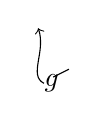
\begin{tikzpicture}[baseline=(g.base)]
\node[inner sep=0pt] (g) at (0,0) {$g$};
\draw[->] (g.west) .. controls +(-.2,.1) and +(.1,-.3) .. (-.17,.7);
\draw (.02,.08)--(.22,.18);
\end{tikzpicture}}-modules simples non isomorphes, et si $K_1$ est une extension de $K$, il n'existe pas de $g_{(K_1)}$-module simple isomorphe à la fois à un sous-$g_{(K_1)}$-module de $M_{1(K_1)}$ et à un sous-$g_{(K_1)}$-module de $M_{2(K_1)}$. (Utiliser a)).

\margin{\P}
5) - On suppose que $K$ est un corps de caractéristique $0$. Soient $V$ un $K$-espace vectoriel de dimension finie, $g=\mathrm{sl}(V)$, $U$ l'algèbre enveloppante de $g$, $U_n$ l'ensemble des éléments de filtration $\leq n$ dans $U$, $U^n$ l'ensemble des éléments symétriques homogènes d'ordre $n$ dans $U$ $(\alpha_1,\ldots,\alpha_m)$ une base de l'espace vectoriel $g$. Soit $W_s=\overset{s}{\bigotimes}V$. La représentation identique de $g$ définit une représentation de $g$ dans $W_s$ qui se prolonge en un homomorphisme $\pi_s$ de $U$ dans l'algèbre $M_s=\mathcal L(W_s)$.
